\documentclass{article}

\usepackage{tikz}
\usepackage{pgfplots}
\usepackage{verbatim}

\usepackage[top=1in, bottom=1.5in, left=1in, right=1in]{geometry}

\usepackage{graphicx}

\author{Stefan Seritan (PERM: 5466644), Wei Dai (CSIL: wdai, PERM: 6925747)}
\date{\today}
\title{CS140 Final Project Progress Report}

\begin{document}
\maketitle

\section*{Serial Results}
\vspace{-7pt}
\indent\indent The Metropolis Monte Carlo simulation for the Potts Lattice Gas (PLG) model was implemented in C++. The melting point and phase diagram for our test system were calculated, as shown below in Figures 1 and 2. The melting point is indicated by the peak in the heat capacity, which is at $kT = 1.35$ for this system. As for the phase diagram, the two phase region ends at $kT = 1.05$. Above this value, the solid can exist as an even mixture, while the solid will split into a species 1 rich phase and a species 2 rich phase within the two phase region (i.e. not perfect mixing). These two values will be used to ensure the algorithm remains formally correct after parallelization.

\vspace{-5pt}
\begin{center}
\textbf{Figure 1.} Heat Capacity ($\frac{dE}{dT}$) vs. Temperature ($kT$)\\
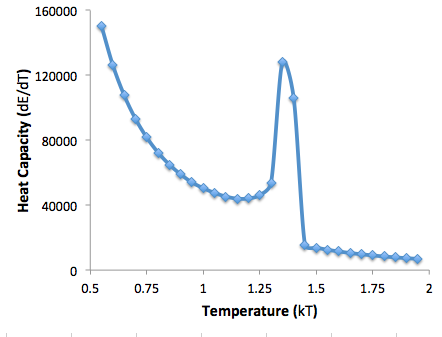
\includegraphics[scale=0.5]{SerialMeltingTemp.png}\\

\vspace{5pt}
\textbf{Figure 2.} Phase Diagram\\
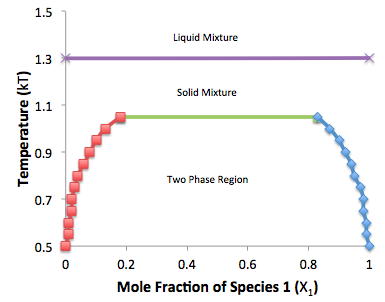
\includegraphics[scale=0.5]{SerialPhaseDiagram.png}\\
\end{center}

\newpage

\section*{Serial Performance}
\vspace{-7pt}
\indent\indent We tested the performance of the serial algorithm on Triton, compiled with icc and -O2 optimization flags. The lattice size we used was $10\times10\times100$, for $100, 500, 1000, 5000, 10000$ equilibration and data sweeps (with $\Theta$ calculated every sweep during data collection). Timing was done using C++11's chrono library. The time needed per sweep and to calculate Theta every sweep is reported below in Figure 3.

\begin{center}
\textbf{Figure 3.} Milliseconds for Sweeps and Theta\\
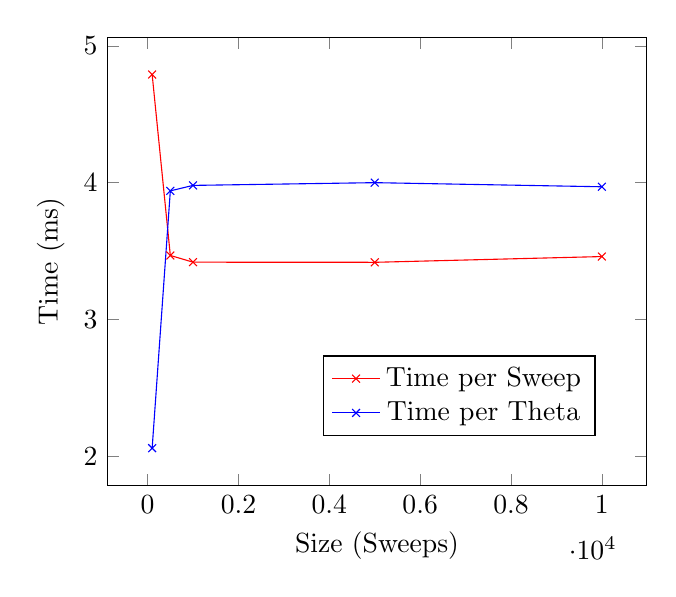
\begin{tikzpicture}
  \begin{axis}[
    xlabel=Size (Sweeps),
    ylabel=Time (ms),
    legend entries={Time per Sweep, Time per Theta},
    legend style={at={(0.4, 0.2)},anchor=west}]
    \addplot[color=red,mark=x] coordinates {
    (100, 4.79)
    (500, 3.468)
    (1000, 3.419)
    (5000, 3.418)
    (10000, 3.460)
  };
      \addplot[color=blue,mark=x] coordinates {
    (100, 2.06)
    (500, 3.94)
    (1000, 3.98)
    (5000, 4.00)
    (10000, 3.97)
  };
  \end{axis}
\end{tikzpicture}
\end{center}

\indent There are a few key insights from the timing information of the serial program. Unsurprisingly, each sweep takes constant time since the lattice size does not change. Therefore, our program is linear in the number of iterations. More importantly, we can see that actually calculating $\Theta$ takes more time than one sweep.

\section*{Parallelizing $\Theta$ Calculation}
\vspace{-7pt}
\indent\indent Parallelizing data collection is theoretically very easy, since it is a 7-point stencil with no data races. We simply wrapped the stencil calculation in cilk\_for's, split up in three dimensional blocks. The size ($n=100,500,1000,5000,10000$ at 16 procs) and processor ($p=1,2,4,6,8,12,16$ for 5000 eq. and data sweeps) scaling was studied using the same chrono timing used for the serial version. Since only $\Theta$ was parallelized at this stage, only the time for $\Theta$ is reported in Figure 4 below.

\newpage

\begin{center}
\textbf{Figure 4.} Parallel Efficiency for Theta Calculation\\
\begin{tikzpicture}
  \begin{axis}[
    xlabel=Procs ($p$),
    ylabel=Parallel Efficiency,
    ymin=0, ymax=1]
    \addplot[color=blue,mark=x] coordinates {
    (1, 1)
    (2, 0.578)
    (4, 0.386)
    (6, 0.296)
    (8, 0.240)
    (12, 0.148)
    (16, 0.124)
  };
  \end{axis}
\end{tikzpicture}
\end{center}

\indent On average, $\Theta$ now only takes over 1 ms to calculate, but it surprisingly scales extremely poorly with increasing processors. We tried several other schemes to iterate over the arrays to increase parallel efficiency, but nothing was very effective. We suspect that perhaps the issue is C++'s internal array implementation. We plan on rewriting the program using a more efficient object oriented approach that will hopefully allow Cilk Plus to more efficiently parallelize the calculation of $\Theta$.

\section*{Parallelizing Move Execution}
\vspace{-7pt}
\indent\indent The other bulk of computational time is actually generating and executing moves. Since the canonical ensemble features the particle swap moves, geometric division cannot be used because almost half of the moves will require communication. Our proposed scheme was to centrally generate moves and then distribute them in independent batches to Cilk to be executed in parallel. This can be done so long as a move does not conflict with moves assigned to 2 processors. Best case scenario for a batch is to do half a sweep, in a checkerboard pattern; however, in reality we find that we can only do approximately 3\% of a sweep before we have to wait for a sync. Since the moves are so lightweight, even the minimal overhead of our separate queues and conflict checking cancels out the gains we get for using multiple cores.\\
\indent We have tested version of the parallel move execution with Cilk Plus, TBB, and OpenMP, but only TBB with the newest compilers on our local machine actually beat the serial version. Again, we believe that our data structures are to blame. We hope that shifting to a better data structure will reduce the overhead of assigning moves and making the parallelization actually worth it.

\section*{Further Parallelization}
\vspace{-7pt}
\indent\indent In addition to the parallelization described above, we can further parallelize the simulation by splitting data sweeps. Assuming the system is at equilibrium, each data sweep simply serves to collect more data about a system that is no longer changing. We could easily split the data sweeps across nodes (potentially using MPI) and have each node collect data independently, only communicating at the very end to average the results. We have not implemented this yet, but it should provide easy scalability.

\end{document}
